\documentclass[conference]{IEEEtran}

% --- Encoding and fonts ---
\usepackage[T1]{fontenc}
\usepackage[utf8]{inputenc}
\usepackage{lmodern}
\usepackage{microtype}

% --- URLs ---
\usepackage{url}
\usepackage{xurl}

% --- Math ---
\usepackage{amsmath}
\usepackage{amssymb}

% --- Tables ---
\usepackage{tabularx}
\usepackage{booktabs}

% --- Graphics ---
\usepackage{graphicx}
\usepackage{tikz}
\usetikzlibrary{arrows.meta, positioning, calc}

% --- Code listings (JSON in Appendix A) ---
\usepackage{listings}
\lstdefinestyle{janusjson}{%
  basicstyle=\ttfamily\footnotesize,
  showstringspaces=false,
  keepspaces=true,
  breaklines=false,
  breakatwhitespace=true,
  columns=fullflexible,
  upquote=true,
  numbers=none,
  frame=single,
  rulecolor=\color{black!18},
  backgroundcolor=\color{black!01},
  framerule=0.3pt,
  framesep=0.7em,
  aboveskip=1.1em,
  belowskip=1.1em,
  xleftmargin=0.5em,
  xrightmargin=0.5em,
}
\lstdefinelanguage{json}{}
\lstset{language=json,style=janusjson}

\title{The Missing Decision Layer: Structural Failure in Information Systems and the Case for a Minimal Governance Kernel}

\author{%
  \IEEEauthorblockN{Martín Nicolás Sánchez Morales}\\
  \IEEEauthorblockA{Janus Governance Project\\
  Buenos Aires, Argentina\\
  ORCID: \url{https://orcid.org/0009-0000-4963-8847}\\
  \url{https://janusgovernance.org}}%
}

\begin{document}

\maketitle

\begin{abstract}
This paper identifies a structural failure in information system design: systems record state changes and the operations that produced them, but do not record --- as a first-class component --- the human decision that authorized each operation. Traditional systems ensure traceability of operations, but not of authorization. The absence of this decision layer produces systems that are not deterministically reconstructible. We term this absence --- and its operational consequences --- the \emph{governance gap}. When the state of a system is contested, the authorization chain that justifies it does not exist within the system. Accountability drifts, and the cost of absent decision records is externalized onto the individuals and institutions that must absorb it.

This failure mode is domain-independent. It has been directly observed across five institutional contexts over four decades, from a national-scale emergency social assistance program to public education administration to AI-assisted software development. The form of the failure is invariant across all five contexts. What varies is the scale of its consequences.

This paper presents the longitudinal evidence for the structural claim, documents the failure modes at institutional scale, and introduces the minimal governance kernel --- formalized in the Janus framework~\cite{sanchez_core,sanchez_framework} --- that restores decision records as a first-class component of the system model. In AI-assisted development contexts, this kernel is not optional: an AI agent operating without a decision layer amplifies the pre-existing structural failure at machine velocity, rendering informal compensatory mechanisms inoperative.
\end{abstract}

\begin{IEEEkeywords}
decision layer, governance gap, governance kernel, structural systems failure, accountability, reconstructibility, AI governance, information systems design, append-only records, evidence model, public administration
\end{IEEEkeywords}

\section{Structural Failure in Information Systems}

Modern information systems are designed around two fundamental components: state and operations. A state change is recorded. The operation that produced it is logged. What is systematically absent from this model is the third required component: the decision --- the human authorization that gave the operation its institutional meaning.

This is not a logging problem. Logs exist. Traditional systems model state transitions, but not the authorization behind them. The failure is architectural: human decisions are not modeled as first-class system components. They are not stored, linked to the state changes they authorized, or made available for downstream reconstruction.

The consequences follow directly from this absence. When a state is contested --- whether in an audit, a legal challenge, a personnel transition, or a system failure --- the system cannot produce the authorization chain that justifies it. Responsibility for outcomes cannot be attributed to specific decisions. It diffuses across the system or onto individuals who must reconstruct it informally. The cost of that reconstruction is transferred to external actors: the person, organization, or institution that must absorb it as operational, legal, or reputational damage. The damage is not generated by the absence of the decision. It was always there, as potential. The absent record makes it irrecoverable.

This structural failure is independent of implementation technology. It has been observed in COBOL-era mainframes, spreadsheet-based administrative systems, relational databases, script-driven workflows, and AI-assisted development environments. What varies across these contexts is the scale and velocity of consequences, not the structural form of the failure.

\subsection{Contributions}

This paper makes three primary contributions:

\begin{enumerate}
  \item It identifies the missing decision layer as a structural failure in information system design, distinct from implementation quality or logging discipline.
  \item It presents longitudinal evidence for this failure as an invariant pattern across five institutional contexts and four decades of direct observation, spanning public administration, social program management, education governance, software development, and AI-assisted production.
  \item It documents the minimal governance kernel --- decision, evidence, accountability --- as the architectural response to the failure, and its alignment with existing governance frameworks~\cite{nist2023,w3c_prov,iso42001}.
\end{enumerate}

\section{Why Systems Are Not Reconstructible}

For a system to be deterministically reconstructible --- meaning: for its current state to be derivable from a verifiable chain of authorized decisions --- the following conditions must hold:

\begin{enumerate}
  \item Every state change must be traceable to an operation.
  \item Every operation must be traceable to a decision.
  \item Every decision must be attributable to an accountable actor.
  \item The record must be append-only and internally auditable.
\end{enumerate}

Most information systems satisfy condition~1. Very few satisfy condition~2. Essentially none satisfy conditions~3 and~4 as a native system property.

When condition~2 fails, a gap opens between what the system records and what actually authorized the change --- the governance gap. It grows with every undocumented decision. When it is encountered operationally, it must be closed by informal means: institutional memory, physical archives, or negotiation between conflicting records. These mechanisms are unreliable, non-transferable, and permanently lost when the individuals who hold them are no longer available.

The structural failure can be stated precisely: a system without a decision layer is not a record of what happened. It is a record of what changed, with the authorization chain stripped out.

\subsection{The AI Amplification Problem}

AI-assisted development does not introduce this failure. It makes it uncontainable.

In human-paced development, the governance gap accumulates at human speed. Informal compensatory mechanisms --- institutional memory, experienced colleagues, organizational documentation --- partially close it. These mechanisms are imperfect, but they operate within the constraints of human time and human process.

In AI-assisted development, three conditions change simultaneously. First, velocity: an AI agent can generate, modify, and deploy artifacts across multiple files and systems within a single session. The governance gap accumulates at machine speed. Second, memory: an AI agent carries no institutional memory between sessions. It operates on the current state of data. If the decision record does not exist in the system, the agent cannot reconstruct it --- outputs may be technically coherent with the current state but institutionally incoherent with the decisions that produced that state. Third, attribution: when an AI agent modifies a system artifact, the authorization chain --- who decided this, why, and with what authority --- becomes structurally more complex and, without a governance layer, invisible.

The informal compensatory mechanisms that partially compensated for the missing decision layer in human-paced systems cannot operate at AI velocity. A pre-existing structural failure becomes a systemic condition.

\section{Longitudinal Evidence Across Institutional Contexts}

The structural failure described above is not a theoretical construct. It has been directly observed across five distinct institutional contexts over four decades of practice --- from the author's first database built at age 9 through public administration, social program management, education governance, software development, and AI-assisted production. The failure mode is invariant across all five contexts.

\subsection{The Invariant Pattern}

Across all five contexts, the following sequence repeats without variation:

\begin{enumerate}
  \item A system is built to manage data.
  \item Humans use it to make decisions over that data.
  \item The data is recorded; the decisions are not.
  \item When data is contested, the decision record does not exist.
  \item Resolution depends on informal memory, physical archives, or negotiation between conflicting systems.
\end{enumerate}

This repetition across contexts constitutes empirical evidence of a structural invariant.

This is a governance architecture failure, not a technology failure~\cite{trist1951}. Each instance was addressed with a local technical response: a script, a parallel database layer, a management application, a dashboard. None resolved the underlying condition because none addressed its structural source. When a problem reproduces itself across contexts, tools, and decades without variation, patching individual symptoms does not eliminate the failure mode --- it relocates it. The required response is structural: introduction of the minimal irreducible layer the system was always missing.

\subsection{National Scale: Emergency Social Assistance (2000--2001)}

The most consequential documented instance occurred at the Ministerio de Trabajo, Empleo y Seguridad Social of Argentina, under a PNUD technical assistance engagement initiated in 2000~\cite{pnud2001}. The engagement was triggered because the Ministry's data systems were already failing under normal operational load. When Argentina entered its worst economic crisis in modern history in 2001, those failures became acute.

The operational mandate was to load the \emph{Programa Jefes y Jefas de Hogar} --- an emergency social assistance program for unemployed heads of household. An initial assessment of the existing system produced the following diagnosis: Visual Basic interfaces connected to an Access database of hundreds of interconnected tables, with no documented schema, no capacity for bulk operations, and no reversibility mechanism. Normal data entry was projected to require more than five years to load one million beneficiaries. The institutional target was two million.

The system the Ministry had in place was not a system that could be operated under emergency conditions. It could not be understood without full reconstruction. It had no reversibility. It accepted unvalidated identifiers. It could not reconcile its records against external authoritative sources.

The operational response was to build a parallel technical layer: a mirror database enabling safe analysis and testing, and providing a restoration point against cascading failures in the undocumented table structure. Data collection was decentralized to a crisis committee of organizations, each submitting beneficiary records in available formats --- spreadsheets, CDs, plain text. These were normalized to a common format, loaded into a staging table, and validated using a CUIL verification algorithm to ensure identifier integrity. The validated set was cross-referenced against the ANSES database to exclude individuals already receiving income from other programs, then imported to the liquidation system. By the second month, over one million beneficiaries were active.

The parallel layer resolved the operational emergency. It did not resolve the structural problem. Every step of that intervention was a manual substitute for a governance layer that did not exist. Every authorization decision made during that intervention --- the choice of technical approach, the validation methodology, the cross-reference protocol --- was never recorded anywhere. The authorization chain for every operational decision made during a crisis affecting one million people is permanently unrecoverable.

This is the structural failure in its most consequential form. The damage was not produced by a technical defect. It was produced by the systematic absence of decision records at a scale where informal reconstruction is not an option.

\subsection{Municipal and Provincial Administration (2004--2025)}

The same structural pattern was encountered across subsequent institutional contexts. In the Municipio de Marcos Paz, three consecutive roles over seven years --- including Subsecretario de Modernización del Estado --- involved direct development of management software for social programs. Each system built to address a governance symptom at the program level reproduced the underlying condition at the management level: state was recorded, decisions were not.

In the DGCyE ecosystem, the same pattern appeared at provincial education administration scale. The direct predecessor implementations of the Janus governance layer were developed at the Secretaría de Asuntos Docentes of Morón (2024--2025), where the structural failure was observable in real-time operation across multiple intersecting systems. This context is documented in detail in Section~IV.

The significance of the five-context, four-decade observation is methodological: the same failure mode, in the same structural form, across five different institutional levels, technology stacks, and administrative domains. This is not a case-specific finding. It is a pattern characteristic of how information systems are currently designed.

\section{Institutional Case: Public Education Administration}

The Secretaría de Asuntos Docentes of Morón, operating within the DGCyE ecosystem, provides a well-documented current instance of the structural failure at institutional scale. The DGCyE administers one of Argentina's largest public education systems, spanning the province of Buenos Aires. The local secretariat operates entirely within Google Workspace, with no dedicated database infrastructure at the local level.

\subsection{Context and Prior Implementations}

Before the formalization of the governance layer, the following operational systems were implemented and deployed: a digital intake system in AppSheet with automated functions and a query-routing interface; a script-driven interface connecting Google Sheets to PDF records for teacher movement histories, enabling retrieval by national identifier; and dashboards for vacancy visualization. These systems functioned operationally. They also reproduced, at a higher level of integration, the same structural failure they were designed to address.

\subsection{Failure Modes at Institutional Scale}

\noindent\textbf{Data-interface-log conflation.} A single Google Sheet serves simultaneously as database, user interface, operation log, and editing surface. No architectural separation exists between these functions. A change to a record is indistinguishable, within the system, from a correction, an administrative decision, or a data entry error.

\medskip
\noindent\textbf{Decision invisibility.} The system records who edited a cell. It does not record why. The institutional decision that authorized the change --- a transfer, a leave of absence, a titularization --- is absent from every component of the system.

\medskip
\noindent\textbf{Cross-system incoherence.} Salary data is managed by a COBOL-era system. Administrative-pedagogical and movement data lives in the provincial ABC system. Statistical platforms operated by other provincial bodies remain disconnected from both --- dashboards that require manual export cycles rather than automated feeds. Administrative codes differ between systems, defined in different decades with no shared schema governance. No system-native reconciliation mechanism exists for resolving discrepancies.

\medskip
\noindent\textbf{Architectural fragility.} Any modification to one component --- a schema change, a new field, a script update --- can propagate failures across the entire system with no traceable record of what changed or why. Each intervention carries systemic risk disproportionate to its apparent scope.

\medskip
\noindent\textbf{Retirement vulnerability.} A teacher's retirement process requires a complete, coherent movement history. Discrepancies between the COBOL system and ABC records cannot be resolved through any system-native mechanism. Resolution depends on human memory and physical archives --- both of which degrade with time and personnel change.

\medskip
\noindent\textbf{Continuity failure.} When administrative personnel change --- as occurs with every electoral cycle in Argentine public administration --- institutional memory that exists only in the departing administrator's personal knowledge is permanently lost. No system component captures the decisions that knowledge represented.

\subsection{Structural Diagnosis}

These six failure modes are not independent defects. They are manifestations of the same missing layer. Introducing any new tool without a decision layer produces a new instance of the same problem at a higher level of integration. The required response is not infrastructure replacement. It is introduction of a governance layer over the existing infrastructure --- one that can operate on top of Google Sheets, Apps Script, AppSheet, and Google APIs without requiring abandonment of any current system component.

\section{Experimental Case: The 3D Dice}

\subsection{Context}

A Three.js 3D dice component was developed as part of a trivia module for an educational platform, operating under Janus governance protocols. This context constituted the first complete production test of the framework under increased rendering complexity.

\subsection{The Problem and Its Resolution}

The component exhibited the following structural condition: the rotation engine calculated face positions in a coordinate space defined by the rendering engine; visual output was determined in a separate representation space. The value produced by the calculation logic did not match the face presented to the user.

Two representations of the same state in disagreement, with no system-native mechanism to determine which was authoritative. This is structurally identical to decision invisibility: a system records a state change but the record contains no information about which representation is correct or what authorized the transition to that state.

The resolution was instrumentation: console telemetry was used to observe actual runtime state at the exact point of discrepancy. Variables were rewritten from observed values, not inferred from visible behavior. This is E\textsuperscript{+} evidence in direct application --- a verifiable record of actual system state replacing inference from output.

\subsection{Chronological Evidence}

The following timeline is reconstructed from git history. All timestamps are independently verifiable.

\begin{table}[t]
\centering
\caption{Chronological evidence from git history (2026-03-21 to 2026-03-23).}
\label{tab:chrono}
\small
\setlength{\tabcolsep}{3pt}
\renewcommand{\arraystretch}{1.08}
\begin{tabularx}{\columnwidth}{@{}>{\raggedright\arraybackslash}p{0.24\columnwidth} >{\raggedright\arraybackslash}p{0.18\columnwidth} >{\raggedright\arraybackslash}X@{}}
\toprule
\textbf{Timestamp} & \textbf{Commit} & \textbf{Event} \\
\midrule
2026-03-21 22:36 & \texttt{42df8b0} & Animated dice integrated \\
2026-03-21 23:02--23:56 & \texttt{00943a6}--\texttt{f70a54f} & Four correction commits in 54~min \\
2026-03-22 00:04 & \texttt{b28e51d} & Simplify to single-axis deterministic rotation \\
2026-03-22 10:21 & \texttt{84b0533} & True random values, decouple from input state \\
2026-03-23 10:40 & \texttt{4fd8261} & Introduce deterministic change-governance layer \\
2026-03-23 22:56 & \texttt{92f639d} & Stabilize 3D dice, fix NaN rotation bug \\
\bottomrule
\end{tabularx}
\end{table}

The governance tooling was formalized on March~23 --- after the problem was encountered on March~21--22. This sequence is evidentially significant: the tool was not designed for a hypothetical scenario. It was built in direct response to a specific, encountered failure, under the same governance protocol it was designed to implement.

\section{Minimal Governance Kernel}

In this paper, three closely related terms are used with distinct referents: \emph{decision layer} names the missing primitive in the current system model; \emph{governance layer} names its introduction as an architectural overlay over existing infrastructure; and \emph{governance kernel} names its minimal formalization, specified in~\cite{sanchez_core,sanchez_framework}.

\subsection{The Missing Layer}

The conventional system model includes two components (state and operations only):

\begin{itemize}
  \item \textbf{State:} the current values held by the system.
  \item \textbf{Operations:} the transformations that modify state.
\end{itemize}

This model is sufficient for recording what changed. It is structurally insufficient for recording why --- for maintaining the authorization chain that gives state changes their institutional meaning.

The Janus framework introduces three additional components:

\begin{itemize}
  \item \textbf{Decision:} the human authorization event that sanctioned the operation.
  \item \textbf{Evidence:} the verifiable classification of whether the expected operation occurred --- E\textsuperscript{+} (occurred as expected) or E\textsuperscript{$-$} (absent, recorded as \texttt{OMISSION\_DETECTED}).
  \item \textbf{Accountability:} the binding between a specific human actor, a specific decision, and a specific state change, recorded in an append-only log that is not retroactively modifiable.
\end{itemize}

These three components constitute the minimum required for the system to be deterministically reconstructible. They are not features added to systems. They are primitives missing from the system model~\cite{kooi2003} --- the layer whose absence produces the structural failure documented in this paper.

\begin{figure}[t]
\centering
\resizebox{0.70\columnwidth}{!}{%
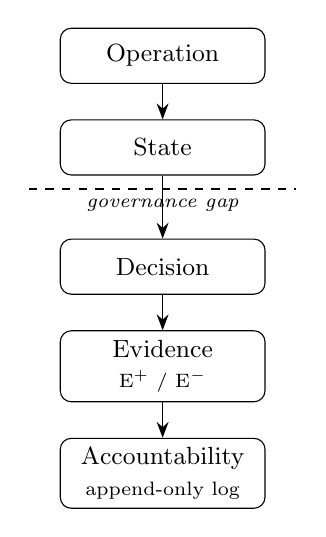
\begin{tikzpicture}[
  node distance=0.45cm,
  kbox/.style={draw, rounded corners, minimum width=2.6cm, minimum height=0.7cm, align=center, font=\small},
  arrow/.style={-Stealth, semithick}
]
  \node[kbox] (op) {Operation};
  \node[kbox] (state) [below=of op] {State};
  \node[kbox] (dec) [below=of state, yshift=-0.35cm] {Decision};
  \node[kbox] (ev)  [below=of dec]  {Evidence\\ {\scriptsize E\textsuperscript{+} / E\textsuperscript{$-$}}};
  \node[kbox] (acc) [below=of ev]   {Accountability\\ {\scriptsize append-only log}};

  \draw[arrow] (op)    -- (state);
  \draw[arrow] (state) -- (dec);
  \draw[arrow] (dec)   -- (ev);
  \draw[arrow] (ev)    -- (acc);

  % governance gap boundary
  \draw[dashed, thick] ($(state.south)+(-1.7,-0.17)$) -- ($(state.south)+(1.7,-0.17)$);
  \node[font=\scriptsize\itshape] at ($(state.south)+(0,-0.38)$) {governance gap};
\end{tikzpicture}
}
\caption{The minimal governance kernel over the conventional (State, Operations) model. Decision, Evidence, and Accountability are introduced as first-class components. The dashed boundary marks the governance gap: the point at which conventional system models terminate and the missing layer begins.}
\label{fig:kernel}
\end{figure}

\subsection{The Formal Invariant}

The central invariant of the governance kernel is:

\medskip
\noindent\emph{Every datum must be bound to the decision that authorized it, and that binding must be internally auditable as a guarantee of deterministic reconstruction.}

\medskip
This invariant is domain-independent. It applies to a spreadsheet cell, a database record, a code artifact, or an AI-generated output. Any system in which this invariant does not hold is not a record of what happened. It is a record of what changed, with the authorization chain stripped out.

\subsection{Implementation Surface}

The kernel is not a replacement for existing infrastructure. It introduces a governance layer that can operate over existing systems --- spreadsheets, relational databases, version control systems, AI-assisted development environments --- without requiring migration or abandonment of existing tools.

The kernel materializes as three components: an \textbf{append-only event log} (\texttt{janus\_events.jsonl}) recording all governance events; an \textbf{evidence model} classifying each expected event as E\textsuperscript{+} or E\textsuperscript{$-$}/\texttt{OMISSION\_DETECTED}; and a \textbf{\texttt{HUMAN\_DECISION} record} capturing the actor, authorization context, and rationale for any operation that advances system state.

The formal specification of the kernel --- its canonical logs (\texttt{MANAGEMENT\_LOG}, \texttt{SCHEMA\_LOG}, \texttt{AUDIT\_LOG}), invariants, and reconstruction equations --- is given in~\cite{sanchez_core}. The operational stack, runtime events (\texttt{OMISSION\_DETECTED}, \texttt{HUMAN\_DECISION}), and the evidence-based conformance benchmark (Event Capture Rate, Governance Verdict Latency, Protocol Violation Detectability Rate) are specified in~\cite{sanchez_framework}. Example event payloads are provided in Appendix~\ref{app:events}.

\subsection{From Pattern to Formalization}

The kernel did not emerge from a design exercise. It crystallized from the same sequence that produced the problem:

A structural failure is encountered in practice. An informal tool is built to work around it. The tool is formalized as a governance component. The component is validated against the original failure. It becomes available for the next context.

The governance core emerged from a script built to address decision invisibility in a spreadsheet system. The framework emerged from needing that script to be reproducible across contexts. Each layer was built because the previous layer exposed its own limitation in a different environment.

The invariant that connects all five observed instances is the same: every operator, administrator, and developer always knew that data carried institutional meaning because someone authorized it. That knowledge was present in practice. It was never captured in structure. The governance kernel makes it a first-class property of the system.

\subsection{Operational Interpretation (Non-Normative)}
\label{sec:opinterp}

\emph{This subsection is non-normative. It does not redefine the model specified in Section~VI. It translates that model into an operational reading for software engineers, backend developers, and system implementers. The authoritative model remains as stated above.}

\noindent\textbf{E.1. The Kernel as a Set of Runtime Constraints}

The minimal governance kernel can be read as three constraints imposed over any system that mutates state:

\begin{itemize}
  \item \textbf{C1 --- Decision binding.} No state mutation is admissible unless it carries a reference to a \texttt{decision\_id} that resolves to a previously recorded \texttt{HUMAN\_DECISION} event.
  \item \textbf{C2 --- Append-only evidence.} The governance log is append-only. No event, once written, may be modified or removed. Corrections are themselves new events.
  \item \textbf{C3 --- Omission as evidence.} The absence of an expected operation is not silence; it is an \texttt{OMISSION\_DETECTED} record. A system that emits nothing when it was expected to emit something is not conformant.
\end{itemize}

These three constraints are restatements of the invariant given in Section~VI-B; they add no new requirements.

\noindent\textbf{E.2. Minimal Operational Structures}

At implementation level, the kernel reduces to the following minimal structures:

\begin{itemize}
  \item \textbf{Decision record.} \texttt{decision\_id}, \texttt{actor}, \texttt{timestamp}, \texttt{rationale}. Persisted once, referenced thereafter.
  \item \textbf{Event record.} \texttt{event\_type}, \texttt{timestamp}, \texttt{payload}, \texttt{decision\_id?} (present when the event represents a state mutation; absent for pure evidence events such as omissions).
  \item \textbf{Append-only log.} An ordered, immutable sequence of event records. The order is the authoritative narrative of how the system reached its current state.
\end{itemize}

No additional structure is required for the kernel to be operational. Indices, caches, or materialized views are permissible but are not part of the kernel.

\noindent\textbf{E.3. Preconditions for State Mutation}

For any state mutation to be admissible, the following preconditions must hold:

\begin{enumerate}
  \item There exists a \texttt{decision\_id} that resolves to a \texttt{HUMAN\_DECISION} record in the log.
  \item The mutation event is written to the log before, or atomically with, the state change.
  \item The mutation event carries the \texttt{decision\_id} as a binding field.
\end{enumerate}

Mutations that violate any of these preconditions are not runtime \emph{errors} --- the system can still execute them --- but they are \emph{ungoverned} in the sense of Section~VI. They produce state that cannot be reconstructed to an authorizing decision.

\noindent\textbf{E.4. Traceability Linkage}

Given any value in system state, the reconstruction path is:

\medskip
\noindent\texttt{value} $\rightarrow$ \texttt{mutation event} $\rightarrow$ \texttt{decision\_id} $\rightarrow$ \texttt{HUMAN\_DECISION} record $\rightarrow$ \texttt{actor} + \texttt{rationale}.

\medskip
If any link in this chain is missing, the value is present but unreconstructible. This is the operational signature of the governance gap: not a thrown exception, but a silent dangling reference from data back to authority.

\noindent\textbf{E.5. Scope of This Subsection}

This subsection does not propose a wire format, mandate a storage backend, prescribe a concurrency model, or define error semantics for ungoverned mutations. These decisions belong to concrete implementations. The kernel constrains only what must be recorded and what must be reconstructible.

\section{Implications for AI-Assisted Systems}

Section~II-A established that AI-assisted development does not introduce the structural failure but amplifies it at machine velocity along three axes: production speed, absence of cross-session institutional memory, and diffusion of the attribution chain. The governance kernel directly addresses each.

The append-only log records all governance events regardless of production velocity --- the governance-gap accumulation rate ceases to be a function of human pace. The \texttt{HUMAN\_DECISION} record captures the human authorization that delegated a function to the agent, making the delegation itself a traceable system event: when an AI agent participates in the decision chain, this record is the only mechanism that renders that participation attributable and auditable. The evidence model detects omissions --- cases where an expected governance event did not occur --- and records them as \texttt{OMISSION\_DETECTED}, preserving auditability even when a decision was not formally captured at the time it was made.

The governance gap is not new. AI systems are not its cause. They are the condition under which leaving it unaddressed is no longer operationally viable.

\section{Alignment with Existing Frameworks}

The governance kernel introduced in Section~VI operates at the architectural layer. Existing frameworks governing information systems, AI-assisted development, and institutional traceability operate at the policy, process, or interchange layers. The kernel does not compete with them; it implements, at the level of the system model, the requirements those frameworks formulate at higher levels of abstraction.

\subsection{NIST AI Risk Management Framework}

NIST AI RMF 1.0~\cite{nist2023} defines four core functions --- Govern, Map, Measure, Manage --- as the organizing structure for AI risk management. The \emph{Govern} function requires explicit accountability mechanisms and documentation of decisions affecting AI system development and deployment. The \texttt{HUMAN\_DECISION} record operationalizes this requirement at the level of the artifact: each authorization event is stored as a first-class system component, not as external documentation. The \emph{Map} and \emph{Measure} functions benefit directly from the append-only log, which provides a reconstructible evidentiary base for impact assessment and metric verification.

\subsection{W3C PROV}

The W3C PROV provenance model~\cite{w3c_prov} defines three primitives --- Entity, Activity, Agent --- as the minimum structure for interoperable provenance. These map directly to the kernel's three components: state corresponds to Entity, operation to Activity, and decision to Agent-authorized event. Governance events recorded under the kernel can therefore be serialized as PROV graphs without structural translation, preserving auditability across heterogeneous systems and enabling cross-institutional reconstruction.

\subsection{ISO/IEC 42001:2023}

ISO/IEC 42001:2023~\cite{iso42001}, the international standard for AI management systems, requires documented processes for human oversight and decision traceability. The kernel provides the minimal technical substrate on which conformance to these requirements can be demonstrated: the \texttt{HUMAN\_DECISION} record evidences human oversight at the granularity of individual operations, and the append-only log evidences traceability as a system-native property rather than a documentary layer.

\subsection{Position}

The governance kernel does not replace these frameworks. It addresses a complementary scope: frameworks specify what must be achieved; the kernel specifies the minimum architectural change that makes achievement verifiable at the system level. A system without the decision layer cannot demonstrate conformance with these frameworks except by informal evidence --- which is exactly the failure documented in this paper.

\section{Conclusion}

The central claim of this paper is structural: information systems model state and operations but do not model, as a first-class component, the decision that authorized each operation. The absence of this layer produces systems that are non-reconstructible, where accountability cannot be established from within the system and the cost of absent decision records is externalized.

The evidence spans four decades and five institutional contexts. The most severe instance --- a national-scale emergency social assistance program in 2001, where every authorization decision made during an intervention affecting one million people was never recorded --- establishes the scale of damage attributable to this failure. The experimental instance --- a 3D rendering component resolved through direct instrumentation rather than inference --- demonstrates the same structural form in a compact, git-verified technical context. These are two different kinds of evidence for the same structural claim: the former shows scale of consequence, the latter shows operative logic.

The minimal governance kernel addresses the failure by introducing the missing layer, not by replacing existing infrastructure. The formal invariant is:

\medskip
\noindent\emph{Every datum must be bound to the decision that authorized it, and that binding must be internally auditable as a guarantee of deterministic reconstruction.}

\medskip
In AI-assisted development contexts, this invariant is operationally necessary. A system in which an AI agent can modify state without producing a traceable decision record is a system in which the authorization chain degrades at machine velocity. The governance kernel is the structural response to that condition.

A system that cannot record the decisions that produced its current state cannot be reconstructed. A system that cannot be reconstructed cannot be audited. A system that cannot be audited cannot be governed. A system that does not model decisions cannot model responsibility.

\appendices
\section{Example Governance Events}
\label{app:events}

The following examples illustrate the event forms referenced in Section~VI-C. Schemas conform to the runtime layer defined in~\cite{sanchez_framework} and the canonical event set defined in~\cite{sanchez_core}. Payloads are drawn from the 3D-die experimental instance documented in Section~V so that each record is traceable to a git-verified commit.

\subsection*{A.1 E\textsuperscript{+} --- recorded occurrence}

\begin{lstlisting}[basicstyle=\ttfamily\scriptsize,caption={Example governance event: recorded occurrence (E\textsuperscript{+}).},label={lst:recorded-occurrence}]
{
  "event": "OPERATION_RECORDED",
  "timestamp": "2026-03-22T00:04:12Z",
  "payload": {
    "repository": "lluvia-de-ideas",
    "commit": "b28e51d",
    "artifact": "dice3d.js",
    "change": "simplify to single-axis deterministic rotation"
  }
}
\end{lstlisting}

\subsection*{A.2 E\textsuperscript{$-$} --- recorded omission}

\begin{lstlisting}[basicstyle=\ttfamily\scriptsize,caption={Example governance event: recorded omission (E\textsuperscript{$-$}).},label={lst:recorded-omission}]
{
  "event": "OMISSION_DETECTED",
  "timestamp": "2026-03-21T23:02:47Z",
  "payload": {
    "expected": "rotation invariant check on render tick",
    "observed": null,
    "scope": "dice3d.render()"
  }
}
\end{lstlisting}

\subsection*{A.3 Human authority closure}

\begin{lstlisting}[basicstyle=\ttfamily\scriptsize,breaklines=true,breakatwhitespace=true,columns=fullflexible,caption={Example governance event: human authority closure.},label={lst:human-authority-closure}]
{
  "event": "HUMAN_DECISION",
  "timestamp": "2026-03-23T10:40:05Z",
  "payload": {
    "actor": "M. N. Sanchez Morales",
    "rationale": "Formalize deterministic change-governance layer in response to the failure sequence of 2026-03-21 to 2026-03-22.",
    "binds": ["4fd8261"]
  }
}
\end{lstlisting}

These three records together satisfy the invariant stated in Section~VI-B: each state change (A.1) is bound to a decision (A.3), and the absence of an expected state change is itself recorded as evidence (A.2). The append-only log that holds these records is the structural artifact referenced throughout this paper as \emph{accountability}.

\begin{thebibliography}{8}

\bibitem{sanchez_core}
M.~N. Sánchez Morales, ``JANUS: A Minimal Governance Kernel for Deterministically Reconstructible Human--AI Development Systems,'' Janus Governance Project, Argentina, 2026. DOI: 10.5281/zenodo.18974356.

\bibitem{sanchez_framework}
M.~N. Sánchez Morales, ``Janus Framework: Operational Stack for Governed AI-Assisted Development,'' Janus Governance Project, Argentina, 2026. DOI: 10.5281/zenodo.19239183.

\bibitem{pnud2001}
PNUD Argentina, \emph{Programa Jefes y Jefas de Hogar Desocupados}, Ministerio de Trabajo, Empleo y Seguridad Social, 2001.

\bibitem{trist1951}
E.~L. Trist and K.~W. Bamforth, ``Some Social and Psychological Consequences of the Longwall Method,'' \emph{Human Relations}, 1951.

\bibitem{kooi2003}
J.~Kooiman, \emph{Governing as Governance}. Sage Publications, 2003.

\bibitem{nist2023}
National Institute of Standards and Technology, ``AI Risk Management Framework (AI RMF 1.0),'' NIST, 2023. [Online]. Available: \url{https://www.nist.gov/itl/ai-risk-management-framework}

\bibitem{w3c_prov}
W3C, ``PROV-Overview: An Overview of the PROV Family of Documents,'' W3C Working Group Note, 2013. [Online]. Available: \url{https://www.w3.org/TR/prov-overview/}

\bibitem{iso42001}
International Organization for Standardization, \emph{ISO/IEC 42001:2023 --- Information technology --- Artificial intelligence --- Management system}, ISO, 2023.

\end{thebibliography}

\end{document}
